%!TEX options = -shell-escape

\documentclass[glossy]{beamer}

% Fonts
\usepackage[utf8]{inputenc}
\usepackage{lmodern}
\usepackage[T1]{fontenc}

% Beamer
\useoutertheme{wuerzburg}
\useinnertheme[realshadow,corners=2pt,padding=2pt]{chamfered}
\usecolortheme{shark}

\setbeamertemplate{navigation symbols}{}

% Tikz
\usepackage{tikz}
\usetikzlibrary{tikzmark, arrows, decorations, decorations.pathreplacing}
\tikzset{every picture/.style={font issue=\scriptsize},
         font issue/.style={execute at begin picture={#1\selectfont}}
}

% Minted
\usepackage{minted}
\newminted{cpp}{autogobble, fontsize=\tiny, escapeinside=@@}
\newmintedfile{cpp}{autogobble, fontsize=\tiny, escapeinside=@@}
\newmintinline{cpp}{escapeinside=@@}
\newmintinline{java}{}
\newmintinline{js}{}
\usemintedstyle{vs}

% GraphicX
\usepackage{graphicx}
\graphicspath{{img/}}

% Macros
\newcommand{\cppref}[2]{\href{http://en.cppreference.com/w/cpp/#1}{\underline{#2}}}

% Meta
\title{C++ Boot Camp 1/2}
\author{Jesse Talavera-Greenberg}
\date{}

\begin{document}

\begin{frame}[fragile=singleslide]
  \frametitle{C++ Boot Camp 1/2}
  \framesubtitle{Jesse Talavera-Greenberg}
  \begin{figure}
    \includegraphics[width=.75\columnwidth]{super-punch-out}
    \centering
  \end{figure}
  \begin{tikzpicture}[remember picture, ->, >=stealth, overlay, red, align=left, line width=2mm]
    \draw (3.5cm, 2cm) node [anchor=east] {\shortstack{\huge \textbf{You}}} -> (6.25cm, 3.5cm);
    \draw (8.5cm, 5.75cm) node [anchor=west] {\shortstack{\huge \textbf{C++}}} -> (6.5cm, 5.5cm);
  \end{tikzpicture}
\end{frame}

\begin{frame}[fragile=singleslide]
  \frametitle{Disclaimers}
  \begin{itemize}
    \item I am not the grader for this course.
    \item This boot camp is entirely voluntary.
    \item Any opinions expressed are my own.
    \item I don't know much about DirectX.
    \item Correctness is likely, but \textbf{not guaranteed}.
  \end{itemize}
\end{frame}

\begin{frame}[fragile=singleslide]
  \frametitle{This Week}
  \begin{itemize}
    \item C++ language and standard library
    \item Common traps
    \item Important concepts
    \item Go to \href{www.cppreference.com}{www.cppreference.com} to follow code in-browser
  \end{itemize}
\end{frame}

\begin{frame}[fragile=singleslide]
  \frametitle{The Big Picture}
  \begin{columns}
    \begin{column}{6cm}
      \begin{itemize}
        \item Mix high-level syntax with low-level management
        \begin{itemize}
          \item Most resource management is abstracted away, though
        \end{itemize}
        \item Originally designed for C compatibility
        \item Not your daddy's C++
      \end{itemize}
    \end{column}

    \begin{column}{6cm}
      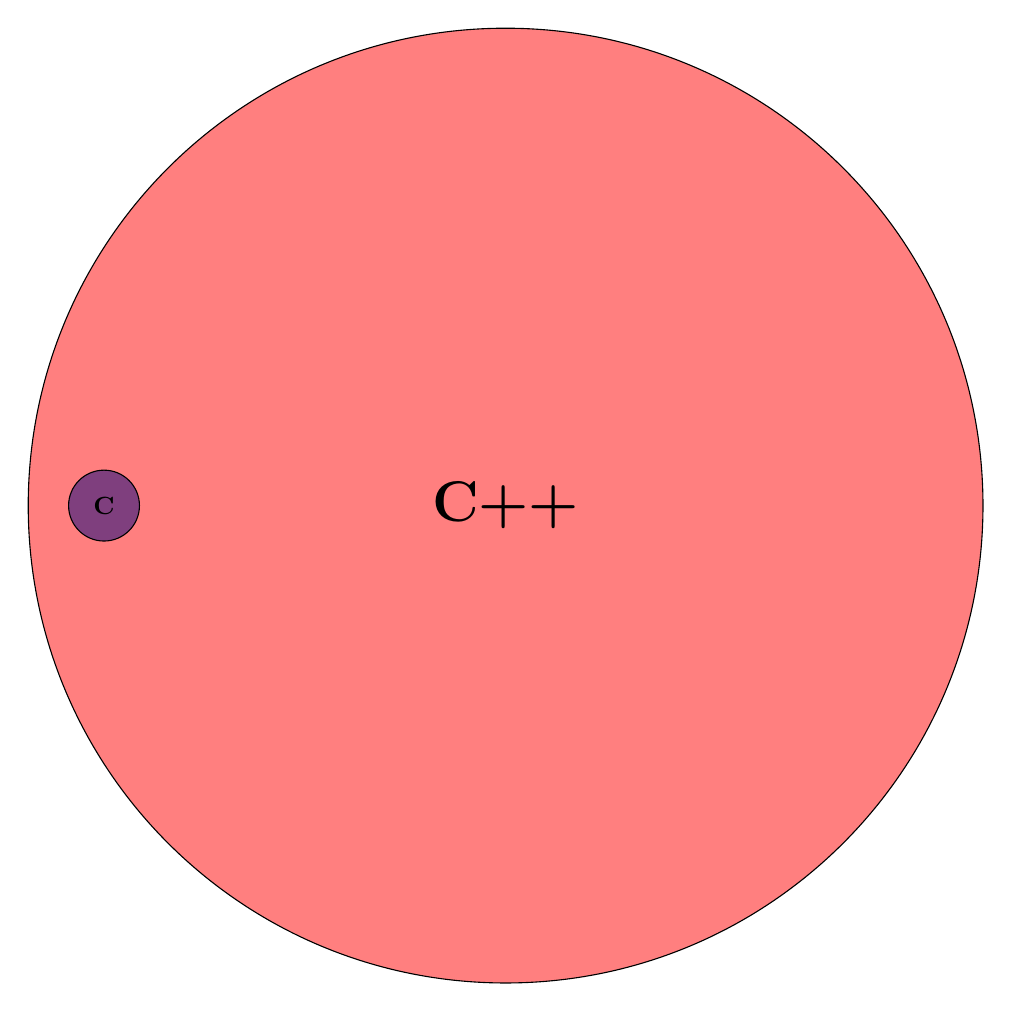
\begin{tikzpicture}[align=center, blend mode=multiply, anchor=center]
        \draw [fill=red, fill opacity=0.5] (0.4\columnwidth,8) circle (0.5\columnwidth) node [fill opacity=1] {\huge{\textbf{C++}}};
        \draw [fill=blue, fill opacity=0.5] (-0.25,8) circle (.45cm) node [fill opacity=1] {\small{\textbf{C}}};
      \end{tikzpicture}
    \end{column}
  \end{columns}
\end{frame}

\begin{frame}[fragile=singleslide]
  \frametitle{\cppref{language/basic_concepts}{The Basics}}
  \cppfile{src/basic.cpp}
  
  
\begin{tikzpicture}[remember picture, ->, >=stealth, overlay, red, ultra thick, align=left]
    \draw (4.5cm, 26em) node [anchor=west] {\shortstack{\cppref{preprocessor/include}{Include libraries, functions, etc.}}} -> ([shift={(.25em,.25em)}]pic cs:basic_include);
    \draw (7cm, 24em) node [anchor=west] {\shortstack{\# of command-line arguments}} -> ([shift={(.25em,.25em)}]pic cs:basic_argc);
    \draw (7cm, 21em) node [anchor=west] {\shortstack{actual arguments as\\a string array}} -> ([shift={(.25em,.25em)}]pic cs:basic_argv);
    \draw[decorate, decoration={brace}, -] ({pic cs:basic_using_a} |- {pic cs:basic_using_b}) +(0,1.5em) -- node [right, inner sep=1em] {Pulls into namespace\\(avoid long-ass prefixes)} ({pic cs:basic_using_a} |- {pic cs:basic_using_b});
    \draw (7cm, 15em) node [anchor=west] {\shortstack{\cppref{io}{Formatted printout}}} -> ([shift={(.25em,.25em)}]pic cs:basic_print);
    \draw (5cm, 3em) node [anchor=west] {\shortstack{Return code (absence in main implies 0)}} -> ([shift={(.25em,.25em)}]pic cs:basic_return);
    \draw (4cm, 12em) node [anchor=west] {\shortstack{Strings not allowed\\in switch statements}} -> ([shift={(.25em,.25em)}]pic cs:basic_switch);
  \end{tikzpicture}
\end{frame}

\begin{frame}[fragile=singleslide]
  \frametitle{\cppref{language/types}{Fundamental Types}}
  \begin{columns}[t]
    \begin{column}{6cm}
      \begin{itemize}
        \item Integer sizes \cppref{language/types\#Data_models}{\textbf{can vary}} by platform, compiler, and OS
        \item No \javainline|byte| (use \cppinline|uint8_t|)
        \item \javainline|boolean| $\rightarrow$ \cppref{language/types\#Boolean_type}{\cppinline|bool|}
        \item Numbers \cppref{language/implicit_cast}{implicitly cast} to \cppinline|bool|
        \item Use \cppref{language/nullptr}{\cppinline|nullptr|} for null pointers, not \javainline|null| or \cppref{types/NULL}{\cppinline|NULL|}
        \item \cppinline|float| and \cppinline|double| exist (also \cppinline|long double|)
      \end{itemize}
    \end{column}

    \begin{column}{6cm}
      \begin{itemize}
        \item \cppinline|signed| and \cppinline|unsigned| integers
        \begin{itemize}
          \item \cppinline|signed| integers are the same
          \item \cppinline|unsigned| go twice as high, but no negatives
        \end{itemize}
        \item For specific sizes, \cppinline|#include @\cppref{preprocessor/include}{<cstdint>}@| and use \jsinline{/std::u?int(8|16|32|64)_t/}
        \item There is \textbf{no} root object class
      \end{itemize}
    \end{column}
  \end{columns}
\end{frame}

\begin{frame}[fragile=singleslide]
  \frametitle{\cppref{language/exceptions}{Exceptions}}
  \begin{cppcode}
#include @\cppref{header/exception}{<exception>}@@\tikzmark{except_header}@
#include <iostream>

using std::cout;
using std::endl;
using std::@\cppref{error/exception}{exception}@;

int couldThrow(int x) {@\tikzmark{except_nocheck}@
  if (x % 2 == 0) throw exception("No new statement (more info later)");
  return x;
}

int willNotThrow(int x) noexcept {@\tikzmark{except_noexcept}@
  return x * x;
}

int main(int argc) {
  int a = willNotThrow(argc);
  try {  
    couldThrow(functionThrow(a));
  }
  catch (exception e)@\tikzmark{except_type}@ {
    cout << e.what();
  }
  catch (...) {@\tikzmark{except_swallow}@
    cout << "What the fuck?";
  }@\tikzmark{except_nofinally}@
}
  \end{cppcode}

  
\begin{tikzpicture}[remember picture, ->, >=stealth, overlay, red, ultra thick, align=left]
    \draw (4cm, 27em) node [anchor=west] {\shortstack{Contains exception handling\\classes and functions}} -> ([shift={(.25em,.25em)}]pic cs:except_header);
    \draw (5cm, 21em) node [anchor=west] {\shortstack{Will not throw an exception\\(program terminates if it does)}} -> ([shift={(.25em,.25em)}]pic cs:except_noexcept);
    \draw (5cm, 9em) node [anchor=west] {\shortstack{Base exception type\\(any type can be thrown, but use these)}} -> ([shift={(.25em,.25em)}]pic cs:except_type);
    \draw (6cm, 4em) node [anchor=west] {\shortstack{No finally statement\\(use destructors instead)}} -> ([shift={(.25em,.25em)}]pic cs:except_nofinally);
  \end{tikzpicture}
\end{frame}

\begin{frame}[fragile=singleslide]
  \frametitle{Type Aliases}
  \begin{cppcode}
#include <array>
#include <cstdint>
#include <iostream>
#include <typeinfo>@\tikzmark{typedef_typeinfo}@

using byte = std::uint8_t;@\tikzmark{typedef_using_a}@

template<class T>
using Array10 = std::array<T, 10>;@\tikzmark{typedef_using_b}@

// Traditional syntax uses "typedef" keyword:@\tikzmark{typedef_prefer}@
//    typedef existing_type new_name;
using std::cout;
using std::endl; 

int main() { 
  std::uint8_t a = 5;@\tikzmark{typedef_okay_a}@
  byte b = a;@\tikzmark{typedef_okay_b}@

  cout << typeid(std::uint8_t).name() << ' ' << typeid(byte).name() << endl;@\tikzmark{typedef_same_a}@

  Array10<byte> c;

  cout << typeid(std::array<byte, 10>).name() << ' ' << typeid(c).name() << endl;@\tikzmark{typedef_same_b}@

  // Many standard types are typedefs (but this is hidden from you)
}
  \end{cppcode}

  
\begin{tikzpicture}[remember picture, ->, >=stealth, overlay, red, ultra thick, align=left]
    \draw (4cm, 22em) node [anchor=west] {\shortstack{Needed for the\\typeid operator}} -> ([shift={(.25em,.25em)}]pic cs:typedef_typeinfo);
    \draw (3cm, 10.5em) node [anchor=west] {\shortstack{Difference is compile-time only}} -> ([shift={(.25em,.25em)}]pic cs:typedef_okay_a);
    \draw (3cm, 10.5em) -> ([shift={(.25em,.25em)}]pic cs:typedef_okay_b);
    \draw (6cm, 16em) node [anchor=west] {\shortstack{Prefer using, but recognize typedef}} -> ([shift={(.25em,.25em)}]pic cs:typedef_prefer);
    \draw (10cm, 11em) node [anchor=south] {\shortstack{Both strings are the same\\(but implementation-defined)}} -> ([shift={(.25em,.25em)}]pic cs:typedef_same_a);
    \draw (10cm, 11em) -> ([shift={(.25em,.25em)}]pic cs:typedef_same_b);
    \draw (6cm, 19em) node [anchor=west] {\shortstack{Another name for\\the same type}} -> ([shift={(.25em,.25em)}]pic cs:typedef_using_a);
    \draw (6cm, 19em) -> ([shift={(.25em,.25em)}]pic cs:typedef_using_b);
  \end{tikzpicture}
\end{frame}

\begin{frame}[fragile=singleslide]
  \frametitle{Memory Model and Lifetime}
  \begin{columns}
    \begin{column}{6cm}
      \begin{itemize}
        \item \textbf{static:} Exists for program's entire duration (on stack or in program data)\tikzmark{memory_static_a}
        \item \textbf{automatic:} Disappears when out of scope (on stack)\tikzmark{memory_auto_a}
        \item \textbf{dynamic:} Created and destroyed at will (on heap)\tikzmark{memory_dynamic_a}
        \begin{itemize}
          \item Remember to clean up (one \cppinline{delete} for every \cppinline{new})
        \end{itemize}
      \end{itemize}
    \end{column}

    \begin{column}{6cm}
      \begin{cppcode}
#include <string>

using std::string;

@\tikzmark{memory_static_b}@string a = "I'll always exist";

void scope() {
  @\tikzmark{memory_auto_b}@string b = "I'll die at the end of the block";
  @\tikzmark{memory_dynamic_b}@string* c = new string("I'll die when you kill me");

  delete c; // c is deleted
  // b is deleted
}

int main() {
  for (int i = 0; i < 100000; ++i) {
    @\tikzmark{memory_dynamic_c}@string* d = new string("Oops");
    // d is not deleted (all 100000 instances of it)
  }

  // a is deleted
}
      \end{cppcode}
    \end{column}
  \end{columns}

  
\begin{tikzpicture}[remember picture, ->, >=stealth, overlay, red, ultra thick, align=left]
    \draw (pic cs:memory_static_a) -> ([shift={(0em,.25em)}]pic cs:memory_static_b);
    \draw (pic cs:memory_auto_a) -> ([shift={(0em,.25em)}]pic cs:memory_auto_b);
    \draw (pic cs:memory_dynamic_a) -> ([shift={(0em,.25em)}]pic cs:memory_dynamic_b);
    \draw (pic cs:memory_dynamic_a) -> ([shift={(0em,.25em)}]pic cs:memory_dynamic_c);
  \end{tikzpicture}
\end{frame}

\begin{frame}[fragile=singleslide]
  \frametitle{Memory Model and Lifetime (cont'd)}
  \begin{columns}
    \begin{column}{6cm}
      \begin{itemize}
        \item Stack allocation is fast, but size must be known at compile time
        \item Heap allocation is flexible, but slow
        \item Details vary by compiler, OS, and hardware
        \item \textbf{All objects of a given type are the same size.}
      \end{itemize}
    \end{column}

    \begin{column}{6cm}
      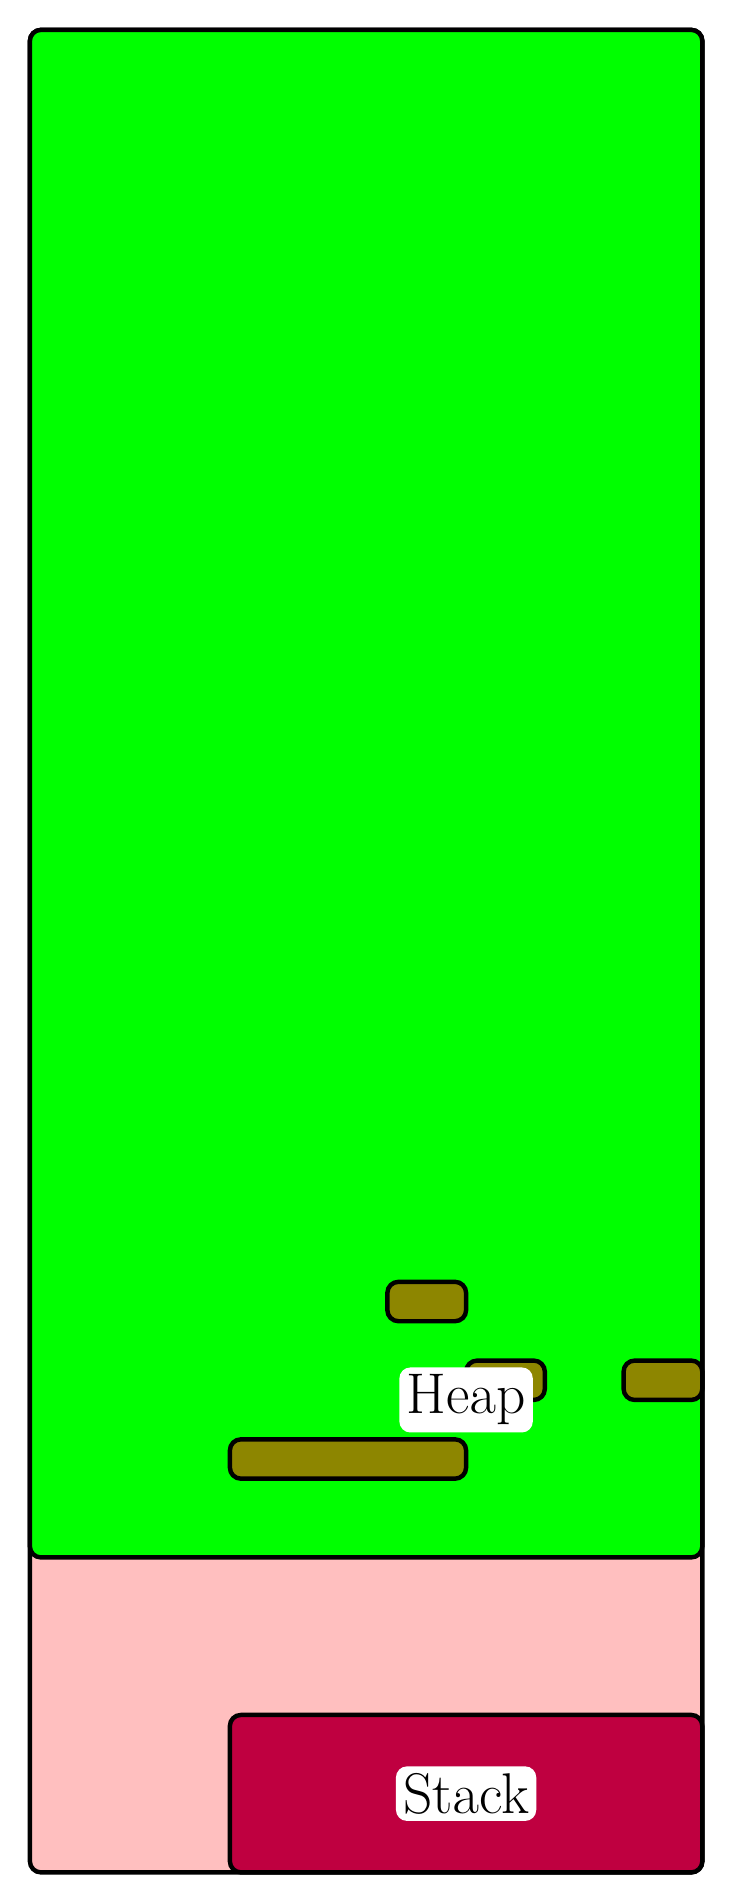
\begin{tikzpicture}[ultra thick, rounded corners]
        \draw [fill=pink] (current page.north west) rectangle (6cm, 2cm);
        \draw [fill=purple] (0cm, 2cm) rectangle (6cm, 4cm) node [align=center, anchor=center, fill=white] at (3cm, 3cm) {\huge{Stack}};
        \draw [fill=green] (current page.north west) rectangle (6cm, 6cm);
        \draw [fill=olive] (2cm, 9cm) rectangle +(1cm, 0.5cm) (3cm, 8cm) rectangle +(1cm, 0.5cm) (5cm, 8cm) rectangle +(1cm, 0.5cm) (0, 7cm) rectangle +(3cm, 0.5cm);
        \draw node [align=center, anchor=center, fill=white] at (3cm, 8cm) {\huge{Heap}};
      \end{tikzpicture}
    \end{column}
  \end{columns}

  \begin{tikzpicture}[remember picture, ->, >=stealth, overlay, red, ultra thick, align=left]
    \draw (4cm, 22em) node [anchor=east] {\shortstack{Find enough space (expensive)}} -> (6.25cm, 5.25cm);
    \draw (4cm, 3em) node [anchor=east] {\shortstack{Increment an address (cheap)}} -> (6.25cm, 1cm);
  \end{tikzpicture}
\end{frame}

\begin{frame}[fragile=singleslide]
  \frametitle{Pointers Vs. References}

  \begin{itemize}
    \item Access lots of data without copying it
    \item Left dangling (\textbf{invalid}) if the referenced object is deallocated
    \begin{itemize}
      \item No way to check for this
      \item Will likely cause a crash if you try to use it
    \end{itemize}
    \item Polymorphism okay
    \item Both compile to similar machine code
    \item Multiple pointers/references can refer to one object
  \end{itemize}

  \begin{columns}
    \begin{column}{6cm}
      \textbf{Pointers:}
      \begin{itemize}
        \item May be invalid (dangling)
        \item Can represent lack of data
        \item Syntax to use and declare
        \item Address can be reassigned
      \end{itemize}
    \end{column}

    \begin{column}{6cm}
      \textbf{References:}
      \begin{itemize}
        \item Always initialized
        \item Points to \textbf{exactly one} address
        \item Less syntax
        \item Easier to deal with objects that shouldn't change
      \end{itemize}
    \end{column}
  \end{columns}
\end{frame}

\begin{frame}[fragile=singleslide]
  \frametitle{Pointers and References}
  \begin{columns}[t]
    \begin{column}{6cm}
      \textbf{Pointers:}
      \begin{cppcode}
#include <iostream>

using std::cout;
using std::endl;

struct Base {
  int enormous[1024];
};

struct Derived : public Base {
  float huge[1024];
};

int main() {
  Base base;
  Derived derived;
  
  Base* a = &base;
  Base* b = &derived; // Polymorphism
  Base* c; // Uninitialized (value undefined)
  c = nullptr;
  c = &derived; // Changed pointer
  
  const Base* d = a; // mutable pointer, const data
  Base const* e = a; // const pointer, mutable data
  const Base* const f = a; // pointer and data const
  
  int* ptr = a->enormous; // Pointer arithmetic
  cout << *ptr << *(ptr + 1) << (*ptr) + 1 << endl;
}
      \end{cppcode}
    \end{column}

    \begin{column}{6cm}
      \textbf{References:}
      \begin{cppcode}
#include <iostream>

using std::cout;
using std::endl;

struct Base {
  int enormous[1024];
};

struct Derived : public Base {
  float huge[1024];
};

int main() {
  Base base;
  Derived derived;
  
  Base& a = base;
  Base& b = derived; // Polymorphism
  // References must be initialized
  // And to a valid object, too
  a = derived; // Changed pointee (the object)
  
  const Base& d = a; // const data
  // References never change (they always point
  // to one address)

  cout << a.enormous[0] << a.enormous[1] << endl;
}
      \end{cppcode}
    \end{column}
  \end{columns}
\end{frame}

\begin{frame}[fragile=singleslide]
  \frametitle{Undefined Behavior}
  \begin{columns}
    \begin{column}{6cm}
      \begin{itemize}
        \item Java fully defines everything
        \item C++ leaves certain edge cases up to the compiler
        \item Many, many ways to invoke
        \item \textbf{Do not rely on UB}
        \begin{itemize}
          \item Best case scenario: Crash
          \item Worst case scenario: No crash
        \end{itemize}
      \end{itemize}
    \end{column}

    \begin{column}{6cm}
      \begin{cppcode}
#include <limits>
#include <string>

using std::numeric_limits;
using std::string;

int something(int param) { 
  if (param > 0) return param; 
  // No return down here; now what? 
} 

string& returnsALocal() { 
  string reference = "Why are you doing this"; 
  return reference; // Uh-oh 
} 

int main() { 
  int a = numeric_limits<int>::max(); 
  a++; // Oops 

  int* pointer; // What's inside?  Beats me.
  int number = *pointer;

  int[10] array; 
  number = array[12]; // WTF 
}
      \end{cppcode}
    \end{column}
  \end{columns}
\end{frame}

\begin{frame}[fragile=singleslide]
  \frametitle{Namespaces}
  \begin{cppcode}
#include <iostream>
#include <string>
#include <array>
#include <utility>

using namespace std;@\tikzmark{namespace_std}@

namespace sbcs {@\tikzmark{namespace_nest_a}@
  namespace cse380 {@\tikzmark{namespace_nest_b}@
    struct Game {
      string name;
      string teamName;
      array<string, 3> members;
    };
  }

  namespace cse381 {@\tikzmark{namespace_nest_c}@
    using Team = pair<string, string>;
  }
}

int main() {
  sbcs::cse380::Game game;@\tikzmark{namespace_qualified}@
  using sbcs::cse381::Team;@\tikzmark{namespace_using}@

  Team team("Jesse", "Karl");
}
  \end{cppcode}

  
\begin{tikzpicture}[remember picture, ->, >=stealth, overlay, red, ultra thick, align=left]
    \draw (6cm, 22em) node [anchor=west] {\shortstack{Don't do this (or java.util.*)}} -> ([shift={(0em,.25em)}]pic cs:namespace_std);
    \draw (5cm, 19em) node [anchor=west] {\shortstack{Nest them as much as you'd like}} -> ([shift={(0em,.25em)}]pic cs:namespace_nest_a);
    \draw (5cm, 19em) -> ([shift={(0em,.25em)}]pic cs:namespace_nest_b);
    \draw (5cm, 19em) -> ([shift={(0em,.25em)}]pic cs:namespace_nest_c);
    \draw (5cm, 8em) node [anchor=west] {\shortstack{Fully-qualified name}} -> ([shift={(0em,.25em)}]pic cs:namespace_qualified);
    \draw (6cm, 4em) node [anchor=west] {\shortstack{Or bring it into the\\current namespace}} -> ([shift={(0em,.25em)}]pic cs:namespace_using);
  \end{tikzpicture}
\end{frame}

\begin{frame}[fragile=singleslide]
  \frametitle{The Preprocessor}
  \begin{cppcode}
#include <iostream>@\tikzmark{cpp_include}@

#define DEBUG@\tikzmark{cpp_define}@

// #define WINDOWS@\tikzmark{cpp_windows}@
// #define MAC@\tikzmark{cpp_mac}@

using std::cout; 
using std::endl; 

int main() { 
  #ifdef DEBUG 
  cout << "Logging! Or sanity checking!" << endl;
  #endif 

  #ifdef WINDOWS
  cout << "Use DirectX!" << endl; 
  #else 
  cout << "Use OpenGL!" << endl; 
  #endif

  #ifndef LINUX@\tikzmark{cpp_linux}@
  cout << "Why do you hate penguins?" << endl;
  #endif

  #ifdef MAC 
    #error "Jesse doesn't like Apple"@\tikzmark{cpp_error}@
  #endif
}
  \end{cppcode}

  
\begin{tikzpicture}[remember picture, ->, >=stealth, overlay, red, ultra thick, align=left]
    \draw (3cm, 25em) node [anchor=west] {\shortstack{Convention: <> for third-party or\\standard library, "" for your code}} -> ([shift={(0em,.25em)}]pic cs:cpp_include);
    \draw (4cm, 21em) node [anchor=west] {\shortstack{Conditional compilation (you can also add\\\#defines through your build process)}} -> ([shift={(0em,.25em)}]pic cs:cpp_define);
    \draw (3cm, 18em) node [anchor=west] {\shortstack{Uncomment these}} -> ([shift={(0em,.25em)}]pic cs:cpp_windows);
    \draw (3cm, 18em) -> ([shift={(0em,.25em)}]pic cs:cpp_mac);
    \draw (4cm, 9em) node [anchor=west] {\shortstack{Contents ignored (not compiled) if on Linux}} -> ([shift={(0em,.25em)}]pic cs:cpp_linux);
    \draw (5cm, 3em) node [anchor=west] {\shortstack{Intentional compiler error}} -> ([shift={(0em,.25em)}]pic cs:cpp_error);
  \end{tikzpicture}
\end{frame}

\begin{frame}[fragile=singleslide]
  \frametitle{Enumerations}
  \begin{cppcode}
#include <iostream> 

using std::cout; 
using std::endl;

enum class Direction {@\tikzmark{enum_not_object}@
  North,
  South,
  East,
  West,@\tikzmark{enum_comma}@
};

enum class Speakers { 
  Mute = 0, @\tikzmark{enum_value}@
  Mono = 1, 
  Stereo = 2, 
  Surround = 4
}; 

enum NaturalBool {@\tikzmark{enum_old}@
  Yes,
  No
};

int main() { 
  Direction dir = Direction::North;@\tikzmark{enum_scoped_a}@
  Speakers audio = Speakers::Stereo;@\tikzmark{enum_scoped_b}@
  NaturalBool yes = Yes;@\tikzmark{enum_unscoped}@

  audio = Speakers(4);@\tikzmark{enum_ub}@
  cout << int(audio) << endl;@\tikzmark{enum_int}@
}
  \end{cppcode}

  
\begin{tikzpicture}[remember picture, ->, >=stealth, overlay, red, ultra thick, align=left]
    \draw (3cm, 25em) node [anchor=west] {\shortstack{Scoped integers, not objects}} -> ([shift={(0em,.25em)}]pic cs:enum_not_object);
    \draw (3cm, 22em) node [anchor=west] {\shortstack{Trailing comma OK}} -> ([shift={(0em,.25em)}]pic cs:enum_comma);
    \draw (3cm, 17em) node [anchor=west] {\shortstack{OK to assign values}} -> ([shift={(0em,.25em)}]pic cs:enum_value);
    \draw (3cm, 13em) node [anchor=west] {\shortstack{Old-style enums\\(recognize, but avoid)}} -> ([shift={(0em,.25em)}]pic cs:enum_old);
    \draw (5cm, 8em) node [anchor=west] {\shortstack{Scoped enum usage}} -> ([shift={(0em,.25em)}]pic cs:enum_scoped_a);
    \draw (5cm, 8em) -> ([shift={(0em,.25em)}]pic cs:enum_scoped_b);
    \draw (5cm, 5em) node [anchor=west] {\shortstack{Avoid if enum is not contiguous}} -> ([shift={(0em,.25em)}]pic cs:enum_ub);
    \draw (4cm, 3em) node [anchor=west] {\shortstack{Explicitly convert enum to int}} -> ([shift={(0em,.25em)}]pic cs:enum_int);
  \end{tikzpicture}
\end{frame}

\begin{frame}[fragile=singleslide]
  \frametitle{Declaring Classes}
  \begin{cppcode}
#include <string>

using std::string;

class Person {
  public:@\tikzmark{class_access_a}@
    int cantBeOverridden(int a, int b) { return this->_integer + b; }@\tikzmark{class_no_override}@
    virtual@\tikzmark{class_virtual}@ float canBeOverridden(double d) { return d * 2; }
    virtual ~Person()@\tikzmark{class_virtual_dtor}@ {}
  protected:@\tikzmark{class_access_b}@
    float _number;
  private:@\tikzmark{class_access_c}@
    int _integer;
};@\tikzmark{class_semicolon}@

struct IBeeGee {@\tikzmark{class_struct}@
  string stayAlive() @\tikzmark{class_abstract}@= 0;
};

class MauriceGibb : public Person, public IBeeGee {@\tikzmark{class_inheritance}@
  void stayAlive() override {
    return "Well, you can tell by the way I use my walk";
  }

  float canBeOverridden(double d) override@\tikzmark{class_override}@ {
    return Person@\tikzmark{class_super}@::canBeOverridden(d) + 23;
  }
};
  \end{cppcode}

  
\begin{tikzpicture}[remember picture, ->, >=stealth, overlay, red, ultra thick, align=left]
    \draw (3cm, 17em) node [anchor=west] {\shortstack{REQUIRED for any inheritable class}} -> ([shift={(0em,.25em)}]pic cs:class_virtual_dtor);
    \draw (3cm, 24em) node [anchor=west] {\shortstack{Access modifiers same as in Java}} -> ([shift={(0em,.25em)}]pic cs:class_access_a);
    \draw (4cm, 12em) node [anchor=west] {\shortstack{struct defaults to public\\class defaults to private}} -> ([shift={(0em,.25em)}]pic cs:class_struct);
    \draw (2cm, 14em) node [anchor=west] {\shortstack{Remember the semicolon!}} -> ([shift={(0em,.25em)}]pic cs:class_semicolon);
    \draw (3cm, 22em) node [anchor=west] {\shortstack{Allows method to be overridden}} -> ([shift={(0em,.25em)}]pic cs:class_virtual);
    \draw (9cm, 19em) node [anchor=west] {\shortstack{Technically you can,\\but things get weird}} -> ([shift={(0em,.25em)}]pic cs:class_no_override);
    \draw (2cm, 11em) node [anchor=north] {\shortstack{Abstract method}} -> ([shift={(0em,.25em)}]pic cs:class_abstract);
    \draw (6cm, 4em) node [anchor=north west] {\shortstack{Marks method as an override\\(optional, but recommended)}} -> ([shift={(0em,.25em)}]pic cs:class_override);
    \draw (2cm, 2em) node [anchor=north] {\shortstack{Call parents with class name}} -> ([shift={(0em,.25em)}]pic cs:class_super);
    \draw (7cm, 7em) node [anchor=west] {\shortstack{Inheritance (actually six\\kinds; just use public)}} -> ([shift={(0em,.25em)}]pic cs:class_inheritance);
  \end{tikzpicture}
\end{frame}

\begin{frame}[fragile=singleslide]
  \frametitle{(Con|De)structors, RAII, and the Rule of 3}
  \begin{cppcode}
#include <cstdint>
#include <cstring>

using std::memcpy;
using std::size_t;

class FloatArray@\tikzmark{raii_dont}@ {
  public:
    FloatArray(size_t size) : _size@\tikzmark{raii_init}@(size), _array(new float[size]) {}@\tikzmark{raii_ctor}@

    FloatArray(const FloatArray& other) : _size(other._size), _array(new float[other._size]) {@\tikzmark{raii_copyctor}@
      memcpy(_array, other._array, other._size * sizeof@\tikzmark{raii_sizeof}@(float));
    }

    FloatArray& operator=(const FloatArray& other) {@\tikzmark{raii_copyeq}@
      if (this != &other) { // Watch for self-assignment!
        float* temp = new float[other._size];
        memcpy(temp, other._array, other._size * sizeof(float));
        delete[] _array;
        _array = temp;
        return *this;
      }
    }

    ~FloatArray() {@\tikzmark{raii_dtor}@
      delete[] floats;@\tikzmark{raii_dtor_b}@
    }

  private:
    size_t _size;
    float* _array;
};
  \end{cppcode}
  
\begin{tikzpicture}[remember picture, ->, >=stealth, overlay, red, ultra thick, align=left]
    \draw (3cm, 27em) node [anchor=west] {\shortstack{Don't write this class\\(STL does it better)}} -> ([shift={(0em,.25em)}]pic cs:raii_dont);
    \draw (5cm, 23em) node [anchor=south] {\shortstack{Member initialization syntax}} -> ([shift={(0em,.25em)}]pic cs:raii_init);
    \draw (8cm, 22em) node [anchor=south west] {\shortstack{Anything else\\(nothing right now)}} -> ([shift={(0em,.25em)}]pic cs:raii_ctor);
    \draw (9cm, 7em) node [anchor=north] {\shortstack{Rule of 3: You need to write one,\\you need to write them all}} -> ([shift={(0em,.25em)}]pic cs:raii_copyctor) node [pos=.5, above, sloped, anchor=north] {Copy constructor};
    \draw (9cm, 7em) -> ([shift={(0em,.25em)}]pic cs:raii_dtor) node [pos=.5, above, sloped, anchor=north] {Destructor};
    \draw (9cm, 7em) -> ([shift={(0em,.25em)}]pic cs:raii_copyeq) node [pos=.5, above, sloped, anchor=north] {Copy assignment};
    \draw (4.5cm, 3em) node [anchor=north] {\shortstack{RAII: Create in ctor, delete in dtor}} -> ([shift={(0em,.25em)}]pic cs:raii_dtor_b);
  \end{tikzpicture}
\end{frame}

\begin{frame}[fragile=singleslide]
  \frametitle{Deleted Functions}
  \begin{cppcode}
#include <cstdint>

using std::size_t;

class FloatArray {
  public:
    FloatArray(size_t size) : _size(size), _array(new float[size]) {}

    FloatArray(const FloatArray&) = delete;@\tikzmark{deleted_a}@
    FloatArray& operator=(const FloatArray&) = delete;@\tikzmark{deleted_b}@

    ~FloatArray() {@\tikzmark{deleted_cleanup}@
      delete[] floats;
    }

  private:
    size_t _size;
    float* _array;
};

int main() {
  FloatArray stack(64);@\tikzmark{deleted_should}@

  FloatArray* heap = new FloatArray(42);
  delete heap;
  // No memory leaks here (or in the previous slide)!
}
  \end{cppcode}
  
\begin{tikzpicture}[remember picture, ->, >=stealth, overlay, red, ultra thick, align=left]
    \draw (8cm, 18em) node [anchor=west] {\shortstack{Forbids this special method\\(compiler error if used)}} -> ([shift={(0em,.25em)}]pic cs:deleted_a);
    \draw (8cm, 18em) -> ([shift={(0em,.25em)}]pic cs:deleted_b);
    \draw (4cm, 14em) node [anchor=west] {\shortstack{Still gotta clean up}} -> ([shift={(0em,.25em)}]pic cs:deleted_cleanup);
    \draw (4cm, 6em) node [anchor=west] {\shortstack{This is how you should use RAII}} -> ([shift={(0em,.25em)}]pic cs:deleted_should);
  \end{tikzpicture}
\end{frame}

\begin{frame}[fragile=singleslide]
  \frametitle{\cppinline{unique_ptr}}
  \begin{cppcode}
#include <cstdint>
#include <memory>

using std::size_t;
using std::unique_ptr;@\tikzmark{unique_ptr}@

class FloatArray {
  public:
    FloatArray(size_t size) : m_size(size), m_array(make_unique@\tikzmark{unique_multiple}@<float[]>(size)) {}

  private:
    size_t m_size;
    unique_ptr<float[]> m_array;@\tikzmark{unique_delete}@
};

int main() {
  FloatArray stack(64);

  FloatArray* heap = new FloatArray(42);
  delete heap;
  // No memory leaks here (or in the previous slide)!
}
  \end{cppcode}
  
\begin{tikzpicture}[remember picture, ->, >=stealth, overlay, red, ultra thick, align=left]
    \draw (4cm, 20em) node [anchor=south west] {\shortstack{At most one unique\_ptr\\can manage an address}} -> ([shift={(0em,.25em)}]pic cs:unique_ptr);
    \draw (8cm, 15em) node [anchor=south] {\shortstack{Use make\_unique, not existing\\pointers (else you risk double-deletes)}} -> ([shift={(0em,.25em)}]pic cs:unique_multiple);
    \draw (5cm, 8em) node [anchor=west] {\shortstack{Cleaned up with RAII}} -> ([shift={(0em,.25em)}]pic cs:unique_delete);
  \end{tikzpicture}
\end{frame}

\begin{frame}[fragile=singleslide]
  \frametitle{Casting}
  \begin{cppcode}
#include <iostream>

using std::cout;
using std::endl;

struct Base { 
  virtual ~Base() {}
};

struct Derived : public Base {
  int thing;
};

int main() {
  Base base;@\tikzmark{cast_poly}@
  Derived derived;

  Base* b_base = &base;
  Base* b_derived = &derived;@\tikzmark{cast_upcast_a}@
  Base& base_ref = base;
  Base& derived_ref = derived;@\tikzmark{cast_upcast_b}@
  
  Derived* d1 = dynamic_cast@\tikzmark{cast_dynamic}@<Derived*>(b_derived);@\tikzmark{cast_dynamic_pass}@
  Derived* d2 = dynamic_cast<Derived*>(b_base);@\tikzmark{cast_dynamic_fail}@

  Derived* d3 = static_cast@\tikzmark{cast_static}@<Derived*>(b_derived);@\tikzmark{cast_static_pass}@
  Derived* d4 = static_cast<Derived*>(b_base);@\tikzmark{cast_static_fail}@

  cout << d1 << ' ' << d2 << ' ' << d3 << ' ' << d4 << endl;
  d4->thing = 52;@\tikzmark{cast_ub}@
}
  \end{cppcode}
  
\begin{tikzpicture}[remember picture, ->, >=stealth, overlay, red, ultra thick, align=left]
    \draw (6cm, 21em) node [anchor=west] {\shortstack{Polymorphism can't be done on values,\\must be pointers or references}} -> ([shift={(0em,.25em)}]pic cs:cast_poly);
    \draw (5cm, 16em) node [anchor=west] {\shortstack{Explicit upcasts rarely necessary}} -> ([shift={(0em,.25em)}]pic cs:cast_upcast_a);
    \draw (5cm, 16em) -> ([shift={(0em,.25em)}]pic cs:cast_upcast_b);
    \draw (6cm, 13em) node [anchor=west] {\shortstack{Runtime type check (slow)}} -> ([shift={(0em,.25em)}]pic cs:cast_dynamic);
    \draw (6cm, 12em) node [anchor=west] {\shortstack{Compile-time type assurance (fast)}} -> ([shift={(0em,.25em)}]pic cs:cast_static);
    \draw (6cm, 9em) node [anchor=west] {\shortstack{Pointer to derived (success)}} -> ([shift={(0em,.25em)}]pic cs:cast_dynamic_pass);
    \draw (6cm, 8em) node [anchor=west] {\shortstack{nullptr (failure, exception if a reference)}} -> ([shift={(0em,.25em)}]pic cs:cast_dynamic_fail);
    \draw (6cm, 6em) node [anchor=west] {\shortstack{Pointer to derived (hopefully success?)}} -> ([shift={(0em,.25em)}]pic cs:cast_static_pass);
    \draw (6cm, 5em) node [anchor=west] {\shortstack{Undefined behavior (hopefully success?)}} -> ([shift={(0em,.25em)}]pic cs:cast_static_fail);
    \draw (3cm, 2em) node [anchor=west] {\shortstack{You fucked up!}} -> ([shift={(0em,.25em)}]pic cs:cast_ub);
  \end{tikzpicture}
\end{frame}

\begin{frame}[fragile=singleslide]
  \frametitle{Concepts}

  \begin{itemize}
    \item Named requirements for a type or function
    \begin{itemize}
      \item Kind of like compile-time interfaces
      \item Usually (but not always) impementing certain methods
    \end{itemize}
    \item Types may be used in templates if they do certain things
    \item Future language revisions will integrate them into the syntax
  \end{itemize}

  \textbf{Examples (simplified):}
  \begin{itemize}
    \item \cppinline{EqualityComparable} $\rightarrow$ provides \cppinline{operator==} for equality test
    \item \cppinline{Container} $\rightarrow$ holds objects and manages their memory (via RAII)
    \item \cppinline{SequenceContainer} $\rightarrow$ \cppinline{Container} whose elements are sequential
    \item \cppinline{FormattedOutputFunction} $\rightarrow$ Function that outputs an object to a \cppinline{std::ostream} (like \cppinline{cout})
  \end{itemize}
\end{frame}

\begin{frame}[fragile=singleslide]
  \frametitle{Templates}
  \begin{cppcode}
#include <iostream>
#include <string>
#include <typeinfo>

using std::cout;
using std::endl;
using std::string; 

template<class T>@\tikzmark{template_stl}@
struct Value {@\tikzmark{template_class}@
  using Type = T;@\tikzmark{template_typedef}@
  T data;

  Value(const T& d) : data(d) {}
};

template<class T>@\tikzmark{template_function}@
void printIt(const Value<T>& val) {
  cout << typeid(typename@\tikzmark{template_depend}@ Value<T>::Type).name() << ' ' << val.data << endl; 
}

struct Dummy {};

int main() { 
  Value<string> text("My name is Beavis");@\tikzmark{template_diff_a}@
  Value<int> number(47);@\tikzmark{template_diff_b}@
  Value<Dummy> dummy(Dummy());@\tikzmark{template_diff_c}@

  printIt(text);@\tikzmark{template_function_deduce}@
  printIt(number);
  // printIt(dummy);@\tikzmark{template_no_print}@
}
  \end{cppcode}
  
\begin{tikzpicture}[remember picture, ->, >=stealth, overlay, red, ultra thick, align=left]
    \draw (3cm, 25em) node [anchor=south west] {\shortstack{Standard library uses\\LOTS of templates}} -> ([shift={(0em,.25em)}]pic cs:template_stl);
    \draw (7cm, 22em) node [anchor=west] {\shortstack{Almost anything can be templated}} -> ([shift={(0em,.25em)}]pic cs:template_class) node [pos=.5, above, sloped, anchor=south] {classes};
    \draw (7cm, 22em) -> ([shift={(0em,.25em)}]pic cs:template_typedef) node [pos=.5, above, sloped, anchor=north] {typedefs};
    \draw (7cm, 22em) -> ([shift={(0em,.25em)}]pic cs:template_function) node [pos=.5, above, sloped, anchor=north] {(member )?functions};
    \draw (3cm, 11em) node [anchor=west] {\shortstack{For types that depend on template parameters inside templates}} -> ([shift={(0em,.25em)}]pic cs:template_depend);
    \draw (6cm, 7em) node [anchor=west] {\shortstack{Three different classes\\and chunks of code}} -> ([shift={(0em,.25em)}]pic cs:template_diff_a);
    \draw (6cm, 7em) -> ([shift={(0em,.25em)}]pic cs:template_diff_b);
    \draw (6cm, 7em) -> ([shift={(0em,.25em)}]pic cs:template_diff_c);
    \draw (3cm, 4.5em) node [anchor=west] {\shortstack{Function type parameters can be deduced}} -> ([shift={(0em,.25em)}]pic cs:template_function_deduce);
    \draw (3cm, 3em) node [anchor=west] {\shortstack{Error: No way to print a Dummy}} -> ([shift={(0em,.25em)}]pic cs:template_no_print);
  \end{tikzpicture}
\end{frame}

\begin{frame}[fragile=singleslide]
  \frametitle{\cppinline{assert}/\cppinline{static_assert}}
  \begin{cppcode}
#include <cassert>
#include <type_traits>

// #define NDEBUG@\tikzmark{assert_ndebug}@
// ^ Uncomment this or define it in the build system to disable asserts

using std::is_base_of;
using std::is_same;

template<class T, class U>
void failIfUnrelated() {
  static_assert(
    is_base_of<T, U>::value
    || is_base_of<U, T>::value
    || is_same<T, U>::value,
    "Both types should be the same, or one should be a parent of the other"
  );
}

class Parent {};
class Child : public Parent {};

int main() {
  assert(1 + 1 == 2);@\tikzmark{assert_use}@

  failIfUnrelated<int, int>();@\tikzmark{assert_ok_a}@
  failIfUnrelated<Parent, Child>();@\tikzmark{assert_ok_b}@
  failIfUnrelated<int, Child>();@\tikzmark{assert_error}@
}
  \end{cppcode}

  
\begin{tikzpicture}[remember picture, ->, >=stealth, overlay, red, ultra thick, align=left]
    \draw (3cm, 24em) node [anchor=west] {\shortstack{Standard "debug mode" \#define}} -> ([shift={(0em,.25em)}]pic cs:assert_ndebug);
    \draw (4cm, 8em) node [anchor=west] {\shortstack{Only run in debug builds (don't\\do side effects or error checking)}} -> ([shift={(0em,.25em)}]pic cs:assert_use);
    \draw (6cm, 4em) node [anchor=west] {\shortstack{OK}} -> ([shift={(0em,.25em)}]pic cs:assert_ok_a);
    \draw (6cm, 4em) -> ([shift={(0em,.25em)}]pic cs:assert_ok_b);
    \draw (5cm, 2em) node [anchor=west] {\shortstack{Compiler error, as desired}} -> ([shift={(0em,.25em)}]pic cs:assert_error);
  \end{tikzpicture}
\end{frame}

\begin{frame}[fragile=singleslide]
  \frametitle{\cppinline{const}}
  \begin{cppcode}
#include <string>

using std::string; 

const int SOME_CONSTANT = 34; 
const string ANOTHER_CONSTANT = "More type-safe than macros!"; 

class ConstStuff { 
  public:
    ConstStuff(int i, const string& s) : _data(i), _text(s) {}

    int data() const { return _data; }@\tikzmark{const_nochange}@
    const string& text() const { return _text; }@\tikzmark{const_ref}@
    string& text() { return _text; }@\tikzmark{const_nonconst_ref}@

    void concatenate(const string& str) { this->_text += str; }@\tikzmark{const_nonconst}@

  private: 
    int _data;
    string _text; 
};

int main() {
  ConstStuff a(1, "France");
  const@\tikzmark{const_ub}@ ConstStuff b(2, "Spain");

  a.text()@\tikzmark{const_overload_a}@.append("FR");
  a.concatenate(b.text());
  // b.text()@\tikzmark{const_overload_b}@.append("SP");@\tikzmark{const_no_cat}@
}
  \end{cppcode}
  
\begin{tikzpicture}[remember picture, ->, >=stealth, overlay, red, ultra thick, align=left]
    \draw (9cm, 21em) node [anchor=west] {\shortstack{No side effects\\(aka state changes)}} -> ([shift={(0em,.25em)}]pic cs:const_nochange);
    \draw (9cm, 18em) node [anchor=west] {\shortstack{Immutable reference\\(no state changes)}} -> ([shift={(0em,.25em)}]pic cs:const_ref);
    \draw (9cm, 15em) node [anchor=west] {\shortstack{Mutable reference\\(state changes possible)}} -> ([shift={(0em,.25em)}]pic cs:const_nonconst_ref);
    \draw (8cm, 12em) node [anchor=west] {\shortstack{Side effects}} -> ([shift={(0em,.25em)}]pic cs:const_nonconst);
    \draw (4cm, 11em) node [anchor=west] {\shortstack{Bypassing const through\\tricks is usually UB}} -> ([shift={(0em,.25em)}]pic cs:const_ub);
    \draw (8cm, 3em) node [anchor=west] {\shortstack{const forbids state changes\\(thus won't compile)}} -> ([shift={(0em,.25em)}]pic cs:const_no_cat);
    \draw (6cm, 7em) node [anchor=west] {\shortstack{One name, two overloads\\(chosen by compiler)}} -> ([shift={(0em,.25em)}]pic cs:const_overload_a);
    \draw (6cm, 7em) -> ([shift={(0em,.25em)}]pic cs:const_overload_b);
  \end{tikzpicture}
\end{frame}

\begin{frame}[fragile=singleslide]
  \frametitle{Operator Overloading}
  \begin{cppcode}
#include <iostream> 

using std::cout; 
using std::endl; 
using std::ostream;@\tikzmark{operator_cout}@

struct Vector2 { 
  float x, y;

  Vector2(float x, float y) : x(x), y(y) {}
  // copy assignment and constructor are implicit

  Vector2 operator+(const Vector2& other)@\tikzmark{operator_sensible}@ { 
    return Vector2(x + other.x, y + other.y); 
  } 
}; 

ostream& operator<<@\tikzmark{operator_ostream}@(ostream& out, const Vector2& v) {
  return out << '[' << v.x << ", " << v.y << ']';
}

bool operator==(const Vector2& a, const Vector2& b)@\tikzmark{operator_eq}@ noexcept {
  return a.x == b.x && a.y == b.y;
}

int main() {
  Vector2 a(1, 2); 
  Vector2 b(2, 1); 
  Vector2 c = a + b; 

  cout << c << ' ' << a == b << endl; // [3, 3] false
}
  \end{cppcode}
  
\begin{tikzpicture}[remember picture, ->, >=stealth, overlay, red, ultra thick, align=left]
    \draw (4cm, 25em) node [anchor=west] {\shortstack{cout is a global std::ostream}} -> ([shift={(0em,.25em)}]pic cs:operator_cout);
    \draw (6.5cm, 16em) node [anchor=west] {\shortstack{Make a type printable (technically doesn't\\fully meet FormattedOutputFunction)}} -> ([shift={(0em,.25em)}]pic cs:operator_ostream);
    \draw (7.5cm, 21em) node [anchor=west] {\shortstack{overloads should be sensible}} -> ([shift={(0em,.25em)}]pic cs:operator_sensible);
    \draw (7cm, 12em) node [anchor=west] {\shortstack{Meets EqualityComparable}} -> ([shift={(0em,.25em)}]pic cs:operator_eq);
  \end{tikzpicture}
\end{frame}

\begin{frame}[fragile=singleslide]
  \frametitle{Data Structures}
  \begin{itemize}
    \item Remember to \cppinline{#include <class_name>}!
    \item Prefer \cppinline{std::array<SomeType, Length>} to \cppinline{SomeType[Length]}
    \item Java describes behavior with interfaces, C++ with concepts
  \end{itemize}
  \begin{columns}
    \begin{column}{6cm}
      \begin{itemize}
        \item \cppinline{vector<T>}
        \item \cppinline{deque<T>}
        \item \cppinline{list<T>}
        \item \cppinline{set<T>}
        \item \cppinline{map<T, U>}
        \item \cppinline{unordered_set<T>}
        \item \cppinline{unordered_map<T, U>}
        \item \cppinline{stack<T>}
        \item \cppinline{priority_queue<T>}
      \end{itemize}
    \end{column}

    \begin{column}{6cm}
      \begin{itemize}
        \item \javainline{ArrayList<T>}
        \item \javainline{ArrayQueue<T>}
        \item \javainline{LinkedList<T>}
        \item \javainline{TreeSet<T>}
        \item \javainline{TreeMap<T, U>}
        \item \javainline{HashSet<T>}
        \item \javainline{HashMap<T, U>}
        \item \javainline{Stack<T>}
        \item \javainline{PriorityQueue<T>}
      \end{itemize}
    \end{column}
  \end{columns}
\end{frame}

\begin{frame}[fragile=singleslide]
  \frametitle{String to numbers and back}
  \begin{cppcode}
#include <cstdlib>
#include <string>

using std::size_t; 
using std::stoi;@\tikzmark{stoi_stoi}@
using std::stol; 
using std::stoll; 
using std::string; 
using std::to_string;@\tikzmark{stoi_wstring}@

int main() { 
  int a = stoi("42");@\tikzmark{stoi_a}@
  long b = stol(" 0x09", nullptr, 16);@\tikzmark{stoi_b}@

  size_t first_nonnumeric_char_index;
  long long c = stoll("12lbs", &first_nonnumeric_char_index, 0);@\tikzmark{stoi_c}@
  // base-0 means assume either base 8, 10, or 16 depending on the prefix

  string back = to_string(c);@\tikzmark{stoi_back}@
}
  \end{cppcode}
  
\begin{tikzpicture}[remember picture, ->, >=stealth, overlay, red, ultra thick, align=left]
    \draw (4cm, 17em) node [anchor=west] {\shortstack{sto(i|u?ll?|f|l?d) is available, too}} -> ([shift={(0em,.25em)}]pic cs:stoi_stoi);
    \draw (4cm, 12em) node [anchor=west] {\shortstack{Or std::to\_wstring}} -> ([shift={(0em,.25em)}]pic cs:stoi_wstring);
    \draw (4cm, 10em) node [anchor=west] {\shortstack{a == 42}} -> ([shift={(0em,.25em)}]pic cs:stoi_a);
    \draw (7cm, 8em) node [anchor=west] {\shortstack{b == 9\\(strips whitespace, reads as base-16)}} -> ([shift={(0em,.25em)}]pic cs:stoi_b);
    \draw (8cm, 3em) node [anchor=north] {\shortstack{c == 2\\first\_nonnumeric\_char\_index == 2}} -> ([shift={(0em,.25em)}]pic cs:stoi_c);
    \draw (4cm, 3em) node [anchor=west] {\shortstack{"12"}} -> ([shift={(0em,.25em)}]pic cs:stoi_back);
  \end{tikzpicture}
\end{frame}

\begin{frame}[fragile=singleslide]
  \frametitle{Regexes}
  \begin{cppcode}
#include <iostream>
#include <regex> // Test out regexes at @\href{https://www.regex101.com}{\underline{regex101}}@
#include <string>
#include <vector>

using std::cout;
using std::endl;
using std::regex;
using std::regex_search;@\tikzmark{regex_match}@
using std::smatch;
using std::string;
using std::vector;

int main() {
  regex secret_council("(\\b[plurandy]+\\b ?){2}"@\tikzmark{regex_syntax}@, regex::icase@\tikzmark{regex_flags}@);
  vector<string> members = {"Duran Duran", "Ayn Rand", "Paul Rudd", "Ann Druyan", "Randall Munroe"};

  for (const auto &m : members) {
      cout << m << ": " << regex_search(m, secret_council)@\tikzmark{regex_search}@ << endl;
  }   
 
  smatch member_match;@\tikzmark{regex_smatch_a}@
  for (const auto &m : members) {
    regex_search(m, member_match, secret_council);@\tikzmark{regex_smatch_b}@
    cout << "matches for '" << m << "':" << endl;

    for (size_t i = 0; i < member_match.size(); ++i) {
      cout << "    " << i << ": " << member_match[i]@\tikzmark{regex_access_match}@ << endl;
    }
  }
}
  \end{cppcode}
  
\begin{tikzpicture}[remember picture, ->, >=stealth, overlay, red, ultra thick, align=left]
    \draw (4cm, 23em) node [anchor=west] {\shortstack{search for finding substrings,\\match for matching whole strings}} -> ([shift={(0em,.25em)}]pic cs:regex_match);
    \draw (6cm, 17em) node [anchor=south] {\shortstack{ECMAScript syntax by\\default, but others available}} -> ([shift={(0em,.25em)}]pic cs:regex_syntax);
    \draw (8cm, 16em) node [anchor=west] {\shortstack{Case insensitive flag}} -> ([shift={(0em,.25em)}]pic cs:regex_flags);
    \draw (8cm, 11em) node [anchor=west] {\shortstack{Returns true if a\\match was found}} -> ([shift={(0em,.25em)}]pic cs:regex_search);
    \draw (7cm, 8em) node [anchor=west] {\shortstack{Class to store actual match\\results and positions}} -> ([shift={(0em,.25em)}]pic cs:regex_smatch_a);
    \draw (7cm, 8em) -> ([shift={(0em,.25em)}]pic cs:regex_smatch_b);
    \draw (7cm, 2em) node [anchor=west] {\shortstack{Actually accessing matches}} -> ([shift={(0em,.25em)}]pic cs:regex_access_match);
  \end{tikzpicture}
\end{frame}

\begin{frame}[fragile=singleslide]
  \frametitle{Custom Map Keys}
  \begin{cppcode}
#include <cstdint>
#include <functional>
#include <tuple>

using std::hash;
using std::size_t;
using std::tie;

struct Coordinates {
  int x, y;
};

bool operator<@\tikzmark{map_lt}@(const Coordinates& a, const Coordinates& b) {
  return tie(a.x, a.y) < tie(b.x, b.y);
}

bool operator==@\tikzmark{map_eq}@(const Coordinates& a, const Coordinates& b) {
  return a.x == b.x && a.y == b.y;
}

namespace std {@\tikzmark{map_std}@
  template<> struct hash<Coordinates> {@\tikzmark{map_hash}@
    using argument_type = Coordinates;@\tikzmark{map_arg}@
    using result_type = std::size_t;@\tikzmark{map_result}@

    result_type operator()(const argument_type& s) const {@\tikzmark{map_func}@
      result_type h1(hash<int>()(s.x));
      result_type h2(hash<int>()(s.y));
      return h1 ^ (h2 << 1);
    }
  };
}
  \end{cppcode}
  
\begin{tikzpicture}[remember picture, ->, >=stealth, overlay, red, ultra thick, align=left]
    \draw (6cm, 23em) node [anchor=west] {\shortstack{For use in ordered (tree-based)\\associative containers}} -> ([shift={(0em,.25em)}]pic cs:map_lt);
    \draw (5cm, 13em) node [anchor=west] {\shortstack{For use in unordered (hash-based)\\associative containers}} -> ([shift={(0em,.25em)}]pic cs:map_eq);
    \draw (5cm, 13em) -> ([shift={(0em,.25em)}]pic cs:map_hash);
    \draw (8cm, 9em) node [anchor=west] {\shortstack{Required for std::hash\\specializations}} -> ([shift={(0em,.25em)}]pic cs:map_arg);
    \draw (8cm, 9em) -> ([shift={(0em,.25em)}]pic cs:map_result);
    \draw (8cm, 9em) -> ([shift={(0em,.25em)}]pic cs:map_func);

  \end{tikzpicture}
\end{frame}

\begin{frame}[fragile=singleslide]
  \frametitle{Random Numbers}
  \begin{cppcode}
#include <iostream> 
#include <random> 

using std::cout; 
using std::default_random_engine; 
using std::endl; 
using std::normal_distribution; 
using std::random_device; 

int main() {
  random_device seed;@\tikzmark{random_device}@
  default_random_engine random(seed());@\tikzmark{random_init}@
  normal_distribution<float>@\tikzmark{random_many}@ normal(0, 1); // mean == 0, stddev == 1

  for (int i = 0; i < 100; ++i) {
    cout << normal(random@\tikzmark{random_concept}@) << ' ';
  }

  cout << endl;
}
  \end{cppcode}
  
\begin{tikzpicture}[remember picture, ->, >=stealth, overlay, red, ultra thick, align=left]
    \draw (4cm, 12em) node [anchor=west] {\shortstack{OS/hardware's source of randomness}} -> ([shift={(0em,.25em)}]pic cs:random_device);
    \draw (5cm, 10em) node [anchor=west] {\shortstack{Initialize a PRNG with a seed}} -> ([shift={(0em,.25em)}]pic cs:random_init);
    \draw (6cm, 6em) node [anchor=north west] {\shortstack{LOTS of distributions available\\(did you take AMS 310 yet?)}} -> ([shift={(0em,.25em)}]pic cs:random_many);
    \draw (3cm, 1em) node [anchor=north] {\shortstack{Or use any UniformRandomNumberGenerator\\(including random\_device, but it's slow)}} -> ([shift={(0em,.25em)}]pic cs:random_concept);
  \end{tikzpicture}
\end{frame}

\begin{frame}[fragile=singleslide]
  \frametitle{Formatted Output and String Concatenation}
  \begin{cppcode}
#include <iomanip>
#include <iostream>
#include <sstream>
#include <string>

using std::cout;
using std::endl;
using std::setprecision;@\tikzmark{formatted_modifier}@
using std::string;
using std::stringstream;@\tikzmark{formatted_stringstream}@

int main() { 
  float x = 5.6435221, y = 7.1453634545, z = -23.452354215;

  stringstream coords;

  coords << "DEBUG LOG\n"
    << "\tPosition: [" << setprecision(4) << x << ", " << y << ", " << z << "]\n";

  cout << coords.str() << endl;@\tikzmark{formatted_str}@
}
  \end{cppcode}
  
\begin{tikzpicture}[remember picture, ->, >=stealth, overlay, red, ultra thick, align=left]
    \draw (4cm, 16em) node [anchor=west] {\shortstack{Changes how floats are printed out\\(many modifiers exist)}} -> ([shift={(0em,.25em)}]pic cs:formatted_modifier);
    \draw (4cm, 12em) node [anchor=west] {\shortstack{std::ostream that writes to a string}} -> ([shift={(0em,.25em)}]pic cs:formatted_stringstream);
    \draw (5cm, 2em) node [anchor=north west] {\shortstack{Use stringstream for nontrivial formats (a la printf)\\Use string::operator+ for concatenation\\Use sto(i|u?ll?|f|l?d) for number conversions}} -> ([shift={(0em,.25em)}]pic cs:formatted_str);
  \end{tikzpicture}
\end{frame}

\begin{frame}[fragile=singleslide]
  \frametitle{Iterators}
  \begin{cppcode}
#include <array>
#include <iostream>
#include <string>

using std::array; 
using std::cout; 
using std::endl; 
using std::string; 

int main() { 
  array<string, 5> strings = {"France", "Spain", "China", "America", "Sweden"};

  // No iterators
  for (int i = 0; i < strings.size(); i++) {
    cout << strings[i] << ' ';
  }
  cout << endl;

  // The clunky way (but lets you use adaptors)
  for (auto@\tikzmark{iterator_auto}@ it = strings.begin()@\tikzmark{iterator_ptr}@; it != strings.end(); it++) {
    cout << *it << ' ';
  }
  cout << endl;

  // The C++11 way
  for (const string&@\tikzmark{iterator_ref}@ s : strings) {@\tikzmark{iterator_begin}@
    cout << s << ' ';
  }
  cout << endl;
}
  \end{cppcode}
  
\begin{tikzpicture}[remember picture, ->, >=stealth, overlay, red, ultra thick, align=left]
    \draw (3cm, 13em) node [anchor=west] {\shortstack{Deduce the type\\(for when its name is long)}} -> ([shift={(0em,.25em)}]pic cs:iterator_auto);
    \draw (8cm, 8em) node [anchor=west] {\shortstack{Probably an ordinary pointer\\(but that's not your concern)}} -> ([shift={(0em,.25em)}]pic cs:iterator_ptr);
    \draw (5cm, 5em) node [anchor=west] {\shortstack{Iteratee must provide\\begin and end methods}} -> ([shift={(0em,.25em)}]pic cs:iterator_begin);
    \draw (3cm, 3em) node [anchor=north west] {\shortstack{Remember to iterate by reference\\(and const if not changing the data)}} -> ([shift={(0em,.25em)}]pic cs:iterator_ref);
  \end{tikzpicture}
\end{frame}

\begin{frame}[fragile=singleslide]
  \frametitle{Anonymous functions and \cppinline{<algorithm>}}
  \begin{cppcode}
#include <algorithm>
#include <array>
#include <functional>
#include <iostream>

using std::array;
using std::cout;
using std::endl;
using std::function;
using std::transform;

int main() { 
  array<int, 10> ints = {5, 7, 1, 2, 3, 9, 2, 1, 4, 2};

  function<bool(int)> isEven = [](int n) -> bool@\tikzmark{lambda_return}@ {
    return n % 2 == 0;
  };

  function<void(void)> printInts = [&ints] {@\tikzmark{lambda_parens}@
    for (int i : ints) {
      cout << i << ' ';
    }
    cout << endl;
  };

  printInts();

  transform(ints.@\tikzmark{lambda_begin}@begin(), ints.@\tikzmark{lambda_end}@end(), ints.@\tikzmark{lambda_inplace}@begin(), [&isEven@\tikzmark{lambda_capture}@](int i) {
    return isEven(i) ? i : i * 2;
  }); // ^ Doubles all odd numbers
  printInts();
}
  \end{cppcode}
  
\begin{tikzpicture}[remember picture, ->, >=stealth, overlay, red, ultra thick, align=left]
    \draw (7cm, 18em) node [anchor=west] {\shortstack{Lambda return type\\(omit to deduce)}} -> ([shift={(0em,.25em)}]pic cs:lambda_return);
    \draw (7cm, 14em) node [anchor=west] {\shortstack{Omit parens if there are no arguments}} -> ([shift={(0em,.25em)}]pic cs:lambda_parens);
    \draw (7cm, 9em) node [anchor=south] {\shortstack{Capture ints by reference\\(omit \& for value capture)}} -> ([shift={(0em,.25em)}]pic cs:lambda_capture);
    \draw (3.5cm, 7em) node [anchor=south] {\shortstack{Run over entire ints array}} -> ([shift={(0em,.25em)}]pic cs:lambda_begin);
    \draw (3.5cm, 7em) -> ([shift={(0em,.25em)}]pic cs:lambda_end);
    \draw (6cm, 3em) node [anchor=west] {\shortstack{Output iterator is same as input\\(so it operates in-place)}} -> ([shift={(0em,.25em)}]pic cs:lambda_inplace);
  \end{tikzpicture}
\end{frame}

\begin{frame}[fragile=singleslide]
  \frametitle{Time}
  \begin{cppcode}
#include <chrono> 
#include <iostream> 
#include <thread>@\tikzmark{time_thread}@

using std::chrono::duration_cast;@\tikzmark{time_cast}@
using std::chrono::milliseconds;@\tikzmark{time_duration}@
using std::chrono::system_clock;@\tikzmark{time_clock}@
using std::cout;
using std::endl;
using std::this_thread::sleep_for;

const int FPS = 60;

int main() {
  milliseconds ms_per_frame(1000 / FPS);@\tikzmark{time_ctor}@
  system_clock::time_point start = system_clock::now();

  for (int i = 0; i < 300; i++) {@\tikzmark{time_loop}@
    cout << "Frame #" << i << endl;
    sleep_for(ms_per_frame);
  }

  system_clock::time_point finish = system_clock::now();
  cout << "Elapsed time: " << duration_cast<milliseconds>(end - start).count() / 1000.0f << " seconds\n";
}
  \end{cppcode}
  
\begin{tikzpicture}[remember picture, ->, >=stealth, overlay, red, ultra thick, align=left]
    \draw (4cm, 23em) node [anchor=west] {\shortstack{Threading is a whole new\\can of worms (let's not open it)}} -> ([shift={(0em,.25em)}]pic cs:time_thread);
    \draw (6cm, 20em) node [anchor=west] {\shortstack{Convert between units of time}} -> ([shift={(0em,.25em)}]pic cs:time_cast);
    \draw (7cm, 17em) node [anchor=west] {\shortstack{Really a typedef for a generic duration\\(you can define your own units)}} -> ([shift={(0em,.25em)}]pic cs:time_duration);
    \draw (6cm, 14em) node [anchor=west] {\shortstack{Several types of clocks exist}} -> ([shift={(0em,.25em)}]pic cs:time_clock);
    \draw (7cm, 11em) node [anchor=west] {\shortstack{Durations accept integers (but\\you can define float typedefs)}} -> ([shift={(0em,.25em)}]pic cs:time_ctor);
    \draw (5cm, 6em) node [anchor=west] {\shortstack{Your game's timer can\\(and should) use only std::chrono}} -> ([shift={(0em,.25em)}]pic cs:time_loop);
  \end{tikzpicture}
\end{frame}

\begin{frame}[fragile=singleslide]
  \frametitle{Next Week}
  \begin{itemize}
    \item Compiling and linking code
    \item Dealing with multiple files
    \item Using Visual Studio
    \item Overview of popular C++ tools
    \item Building and using a library
  \end{itemize}
\end{frame}

\end{document}